\documentclass[a4paper,12pt,onecolumn]{article}

\usepackage[english]{babel}
\usepackage{amssymb,amsmath,array,epsfig,a4,subfig}


\newcommand{\errorXx}{\|\Gamma^h - \Gamma\|_{L^\infty}}
\newcommand{\LerrorUu}[1]{\|\vec U - I^h_{#1}\,\vec u\|_{L^2(\Omega_T)}}
\newcommand{\errorUu}[1]{\|\vec U - I^h_{#1}\,\vec u\|_{L^\infty}}
\newcommand{\errorPp}[1]{\|P - I^h_{#1}\,p\|_{L^\infty}}
\newcommand{\LerrorPp}{\|P - p\|_{L^2(\Omega_T)}}

\begin{document}

\captionsetup[subfigure]{labelformat=empty} % remove label subplot
\newcolumntype{H}{>{\setbox0=\hbox\bgroup}c<{\egroup}@{}} % hide table column

\section{Miscellaneous}

\begin{figure}[htbp]
\centering
\includegraphics[width=.45\textwidth]
{figures/2d_stationary_bubble_adaptive_100.ps}
\caption{($\mu=\gamma=1$) Pressure of the 2d stationary bubble at time $t=1$
for the P2--P0 element.}
\end{figure}

\begin{figure}[htbp]
  \centering
  \subfloat[$t=0$]{\includegraphics[width=.45\textwidth]
  {figures/expanding_bubble_uniform_000.ps}}\\
  \subfloat[$t=0.25$]{\includegraphics[width=.45\textwidth]
  {figures/expanding_bubble_uniform_025.ps}}
  \subfloat[$t=0.5$]{\includegraphics[width=.45\textwidth]
  {figures/expanding_bubble_uniform_050.ps}}\\
  \subfloat[$t=0.75$]{\includegraphics[width=.45\textwidth]
  {figures/expanding_bubble_uniform_075.ps}}
  \subfloat[$t=1$]{\includegraphics[width=.45\textwidth]
  {figures/expanding_bubble_uniform_100.ps}}
\caption{($\mu_+ = 10\,\mu_- = \gamma = 1,\alpha = 0.15$) Pressure evolution of
the 2d expanding bubble for the P2--P0 element, $C_r=3$.}
\end{figure}

In order to choose the better remeshing coefficient $C_r$ several experiment
were carried out. Some errors for our approximation are shown in
Table~\ref{tab:expandingbubble2Dp2p0bothdiffcr} with a starting characteristic
length $c_l=0.1$, using P2--P0 polynomials and smoothing coefficient $C_s=1$.
The better result are obtained with $C_r=3$ because it reduces the number of
remeshing compared to $C_r=2$ while keeping the same performance and error
quality. For this reason we are going to use this parameter for the other
simulations.
\begin{table*}
 \center
\begin{tabular}{llHllHll}
\hline
$C_r$ & $\errorXx$ & $\LerrorUu2$ & $\errorUu2$ & $\LerrorPp$ & $\errorPp0$ &
$CPU[s]$ & $K_\Omega^T$\\
\hline
2 & 1.46658e-03 & 1.05801e-04 & 8.73227e-04 & 2.14589e-01 & 3.68834e-02 & 4297
& 452\\
3 & 1.47162e-03 & 1.02085e-04 & 7.19650e-04 & 2.13599e-01 & 3.68834e-02 & 3919
& 468\\
4 & 1.46761e-03 & 1.27330e-04 & 8.55458e-04 & 2.19071e-01 & 3.68834e-02 & 4682
& 504\\
5 & 1.47218e-03 & 1.26419e-04 & 7.20711e-04 & 2.12456e-01 & 3.68834e-02 & 4775&
468\\
\hline
\end{tabular}
\caption{($\mu_+ = 10\,\mu_- = \gamma = 1,\alpha = 0.15$) Expanding bubble
problem on $(-1,1)^2\setminus[-\frac{1}{3},\frac{1}{3}]^2$ over the time
interval $[0,1]$ for the P2--P0 element, $C_s=1$, $c_l=0.1$ and uniform mesh.}
\label{tab:expandingbubble2Dp2p0bothdiffcr}
\end{table*}

Instead, in Figure~\ref{fig:shear_2d_smooth} the remeshing coefficient is
$C_r=0$ so only the smoothing is used. The bulk inner relative volume evolution
is reported in Figure~\ref{fig:shear_2d_smooth_bulk_inner_volume}.
\begin{figure}[htbp]
  \centering
  \subfloat[$t=0.5$]{\includegraphics[width=.45\textwidth]
  {figures/2d_shear_smooth_050.ps}}\quad
  \subfloat[$t=1$]{\includegraphics[width=.45\textwidth]
  {figures/2d_shear_smooth_100.ps}}\\
  \subfloat[$t=2.5$]{\includegraphics[width=.45\textwidth]
  {figures/2d_shear_smooth_250.ps}}\quad
  \subfloat[$t=5$]{\includegraphics[width=.45\textwidth]
  {figures/2d_shear_smooth_500.ps}}\\
  \caption{($\mu=1,\gamma=3$) Pressure evolution of the 2D shear flow with
$c_l=0.05$, $C_s=1$ and no remeshing for the P2--P0 element, uniform mesh.}
  \label{fig:shear_2d_smooth}
\end{figure}

\begin{figure}[htbp]
  \centering
  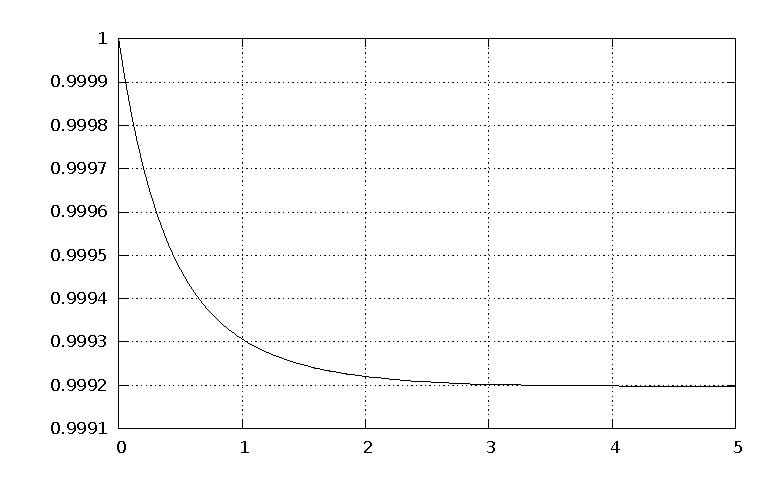
\includegraphics[width=.45\textwidth]
  {figures/2d_shear_smooth_bulk_inner_volume.ps}
  \caption{($\mu=\gamma=1$) Bulk inner relative volume evolution of the 2D
shear flow with $c_l=0.05$, $C_s=1$ and no remeshing for the P2--P0 element,
uniform mesh.}
  \label{fig:shear_2d_smooth_bulk_inner_volume}
\end{figure}

Overall, our proposed method has the following properties.
\begin{itemize}
\item The fully discrete scheme is unconditionally stable in the sense that the
total surface energy is monotonically decreasing independent of the chosen time
step size.
\item In the absence of outer forces, any discrete solution with a stationary
interface must have zero velocity globally, i.e.\ we can prove that there are
no stationary solutions with spurious velocities. Similarly, discrete
stationary solutions for spherical interfaces are attained for our scheme.
\item For the semidiscrete continuous-in-time variant of the fully discrete
scheme the volume of the two phases is conserved. The fully discrete scheme
itself maintains the enclosed volumes well in practice.
\item Thanks to the fitted nature of the finite element method, the pressure
jumps at the interface are captured accurately for standard pressure finite
element spaces without the need for XFEM extensions and no pressure
oscillations appear in practice.
\item The surface tension effects are included with the help of a variational
treatment of curvature based on the Laplace--Beltrami operator.
\item The surface mesh quality is maintained. In particular, for the
semidiscrete scheme an equidistribution property can be shown in 2d.
\item The fully discrete scheme uses an implicit approximation of curvature
that leads to a coupled linear system of equations to be solved at each time
step.
\end{itemize}

\end{document}